\documentclass[14pt]{article}

\usepackage[utf8]{inputenc}

\usepackage{graphicx}	% For figures and similar
\usepackage{amsmath}	% For lots of useful maths tools and characters
\usepackage{amsfonts}	% For fun maths fonts
%\usepackage{pdfpages}

\usepackage[hmarginratio=1:1,top=32mm,columnsep=20pt]{geometry}  % Document margins
\usepackage[hang, small,labelfont=bf,up,textfont=it,up]{caption}  % Custom captions under/above floats in tables or figures
\usepackage{subcaption}
\usepackage{algorithm}
\usepackage{algorithmic}

\usepackage{booktabs}  % Horizontal rules in tables - makes tables look nicer
%\usepackage{hyperref} % For hyperlinks in the PDF
\PassOptionsToPackage{hyphens}{url}\usepackage{hyperref}

\usepackage{fixltx2e} % to use subscripts in normal text

\graphicspath{ {./images/} }

\usepackage{float}


%---------------------------------------------------------------------------------------------------

\title{Mail Delivery}
\author{%
\textsc{Vivian Hogarth, Beth Plummer, Nic Powell} \\[1ex] 
\textsc{Seb Stanbridge, Lewis Vaughan, Miles Weedon} \\ [1ex]
\normalsize Group 4 \\ 
}
\date{\today} 

%------------------------------------------------------------------------------

\begin{document}
\maketitle

\section{Abstract}


%------------------------------------------------------------------------------

\section{Introduction}
This report concerns formulating an algorithm which allows a post-person to calculate the fastest possible route to take when delivering a round of post by telling the post-person how often to move and lock up his cart and to return to the said cart to pick up more mail. The calculation of the best route relies on a series of variables; number of houses requiring mail delivery, spacing between houses, the amount of post the post-person can carry, his walking speed, distribution of suitable street furniture. These variables were all considered  to produce an algorithm which can quantitatively compare the routes based on the completion time. The problem is certainly a relevant one, as it is not only applicable to mail delivery, but could apply in a range of situations requiring the fastest route based on changing variables. For example an emergency vehicle navigating through traffic.
Other studies conducted which are similar to the problem mostly involve the modelling of streets as vertices \textbf{(2)}, and a route between them defined by a ‘traversable graph’\textbf{(1)}, as is done in the ‘Chinese postman problem’. This similarly takes the least distance travelled in total as the best overall route to deliver the mail. This study however takes a broader approach to the issue, whereas our report looks into the finer details which concern deliveries to individuals houses at a time, rather than whole streets.



%------------------------------------------------------------------------------
\section{Methods \& Results}

\subsection{Assumptions}

 To ensure that our method stayed relevant to the question and was simplistic enough that we could develop a simple solution  we set a list of key assumptions:

Assumptions:
\begin{itemize}
    \item Only use one street not connected to others: \\
    To consider multiple streets connected together would make this task too time-consuming, especially as there are no two roads that are the same. 
    \item Straight down one side of the street: \\
    The curvature of a road will be a factor required in calculating when the postman should cross the street. For some routes considered in this report (where the postman delivers to each side of the street in-turn) they will only cross over once; it is therefore appropriate to ignore curvature. It will have an influence on other routes involving more than one cross over, but more time would be needed to account for this in calculations. 
    \item Walks with the same pace with and without the cart: \\
    The difference between the two speeds will be small, causing negligible affects to our final results. 
    \item It takes no time to post the letters through the door: \\
    Total time to post letters to all houses on a street will be a constant, no matter the route the postman takes. Thus, this time has been ignored. 
\end{itemize}

\subsection{First Algorithm}

For our first algorithm the assumptions include:
\begin{itemize}
    \item The distance between each house is the same
    \item The postman carries the same amount of letters each time
    \item Lamp posts are equally spaced
\end{itemize}
 
When writing the code for the first algorithm we started with a simplistic model first:

\begin{algorithm}
\caption{Time to deliver to each house without the cart}
\begin{algorithmic} 
\STATE $time \leftarrow 0$
\STATE $cart\_amount \leftarrow ANY NUMBER$
\STATE $carrying \leftarrow 0$
\WHILE{$cart\_amount \neq 0$}
\IF{$cart\_amount > 5$}
\STATE {$carrying \leftarrow 5$}
\STATE {$cart\_amount \leftarrow cart amount - 5$}
\STATE {$time \leftarrow time + 5$}
\ELSE
\STATE $carrying \leftarrow cart_amount$
\STATE $cart_amount \leftarrow 0$
\STATE $time \leftarrow time + carrying$
\ENDIF
\WHILE{$carrying \neq 0$}
\STATE $time \leftarrow time + time\_to\_walk\_to\_each\_house + time\_to\_deliver\_to\_each\_house$
\STATE $carrying \leftarrow carrying - 1$
\ENDWHILE
\ENDWHILE
\end{algorithmic}
\end{algorithm}


This algorithm found the time to deliver letters to each house assuming that the cart stayed with the postman at all times and it took negligible time for the postman to return to the cart.  The algorithm also assumed that the postman could hold 5 letters and each letter took one second to pick up from the cart.
This first algorithm gave the very simple equation of:
\begin{equation}
    t = P(1+w+d)
\end{equation}

Let t = time (seconds)

Let P = amount of parcels

Let w = time to walk up driveway

Let d = time to walk between houses

If w and d are set as constants then the time to deliver to each house increases linearly with the amount of parcels.
 
The second algorithm that we developed included the postman walking back to the cart each time that he delivers all the post that he is carrying (assumed to be a maximum of 5 in this instance); in this algorithm it is assumed that the cart does not move from its original starting position.

\begin{equation}
    d = 4(P)^2 + 30P
\end{equation}

Let d = distance (metres)

Let P = amount of parcels

for P that is a multiple of 5 assuming that the postman can carry a maximum of 5 letters at once.
This also assumes that the driveway distance is 10m and the distance between houses is 20 metres which can be set as constants at the beginning of the program running. This model is quadratic which is more accurate than the first model that we developed.
 
The third model calculated the time that it would take the postman to make the deliveries if he moved the cart to the lamppost every time he delivered to a house, which set up the method for creating our forth algorithm. For this algorithm we assumed that the postman’s regular walking speed was 1.4m/s and his walking speed with the cart as 2m/s. Each time the postman’s hands were empty he would go back to the cart and move it to the next lamppost then would walk back to the house he was next to deliver to.

\begin{equation}
d = 16/5 P^2 - 6P + 240    
\end{equation}

Let d = distance (metres)

Let P = amount of parcels

\begin{figure}[H]
\centering
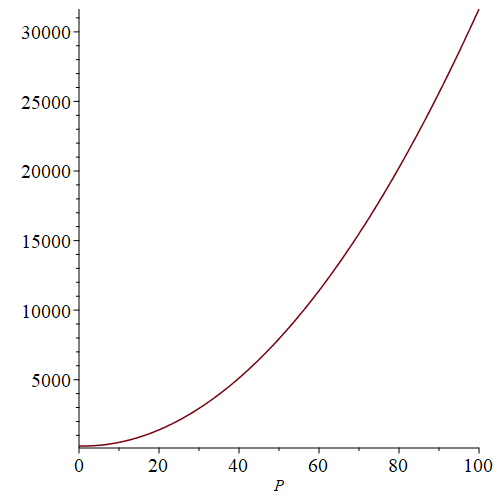
\includegraphics[width = 230pt]{Images/graph.png}
\caption{Updated equation plotted}
\label{fig:equation 3 plot}
\end{figure}

Assuming that the distance between houses is 20 metres and the length of each driveway is 10 metres. The distance does not follow the equation until at least 15 parcels are being delivered.
In this model the time taken for the postman to make all the deliveries would not be equal to the distance / time as the postman has been assumed to have different walking speeds depending on if he is walking with the cart. The time would also be affected by the time it takes the postman to tie up the cart each time he moves it.
For the last two models we have assumed that each house on the street is being delivered to. We have done this so that we can find an equation for the distance in each of the models. If a probability factor is added into the algorithm then answers will not always be produced in a linear or quadratic equation.
 
In our forth model we combined the previous two models and implemented a way to find the distance travelled and time taken if the cart was moved any amount of times. This algorithm iterates through all the possible amounts to move the cart, it calculates the amount of time for each iteration and then compares all the times at the end to find the most efficient cart movements.

\subsection{Three Updated Models}

Using our previous model with some adjustments removes the need to make as many assumptions. For the following models, there is now no need to assume: distance between each house is the same, distance between lampposts are the same and that the postman carries the same amount of post each time. Note that each model is a potential route a postman would follow depending on the street's parameters. 

The length of each house's drive has been ignored in these models. No matter what route is taken, the postman will always take the same time to walk up and down each drive. This is therefore a constant across each model and so is neglected. For this code to work, we have assumed that doors, for all houses, are taken to be at the end of the house's width. An algorithm that took door placement of each house into consideration would make this algorithm too complex. Furthermore, we will assume that the postman can carry just as many parcels as letters. 

Our algorithm is split up into different python modules (see appendix below). This consists of three separate python modules for each of our models. There is also a module which contains data about a number of different streets ("SideOfStreetModels"). We used an init file which acts as our script; it calls upon the other modules to allow us to output our results for comparison for the different streets. It will output a distance travelled to deliver all mail for each street, along with the corresponding time, for each model. Subsequently, this allows us to compare between each of our models. All python files used can be found in the appendix at the bottom of the report. 

The "SideOfStreetModels" module was necessary as it allows the user to enter different parameter values for different streets. The parameters we used consisted of the following:
\begin{enumerate}
    \item Lamppost positions along a side of the road referenced from the start of the road [m]
    \item List of distances between doors of neighbouring houses
    \item House positions along a side of the road referenced from the start of the road [m]
    \item List of number of letters to be delivered to each house on one side of a street
    \item Maximum number of letters the postman can carry at a time
    \item Width of the road
\end{enumerate}

The code for the first model of the three can be found in the "SingleStreetSideNextlampPost" module. This model's code is formatted as one main function (that gets called by the init module).The basis of this code is that the postman, from the start of the road, will first find which lamppost to lock his cart up to. From there he will return to the door of the first delivery house. 

From here, the postman will start delivering to houses up the one side of the street, based on the maximum amount of mail that he can carry at one time. The next step is for him to walk back to the cart. Note that if he locks up and the next 2 houses both have 10 letters that need delivering, but he can only carry 15 letters, he will only deliver to the first house and then return to the cart to get more mail, rather than him getting to the second house, dropping 5 letters off, then going to the cart to get the other 5. Once back at the cart its decided whether the cart needs to be moved or  more mail can be grabbed. In each case, he will then move to the next delivery house, and follow the steps above (from the point where he delivers the mail). These commands for the postman are repeated until the cart is empty. As the postman moves up the street, there are counts for amount of mail delivered and total distance travelled that are continuously updated as the postman moves. Once all mail is delivered to on the one side of the road, he will move the cart to the end of the road and the loop is terminated. 

Note that after delivering to a house there is a vital check in this code to see if the next, neighbouring houses on the street, have any mail to be delivered. If the answer is yes, he will continue on as stated above, carrying as much as he can. If no however, and the next couple of houses have no mail to be delivered, the code checks to see if it is worthwhile for him to keep walking or to move the cart to a better position to shorten his distance travelled. \\
\\
The second model "SingleStreetSideNearestLampPost", is similar in a way to the first; it has the postman walking up one side of the street at a time. It also consists of a main function, that calls upon other functions within. The main difference now is that this model creates a python dictionary. The keys respond to the index of each lamppost on the street from the start point. The values corresponding to each key are lists of 'closest houses', to each lamppost. For instance, if houses of index 0 and 1 are closest to lamppost 0, then the dictionary will start with {0:[0,1], }. These lists of houses only include closest houses that have mail to be delivered, excluding those that don't as there is no need to stop at this lamppost. 

This route is for the postman to first go to the first lamppost. He will lock up and then deliver to all of the associated closest houses in the dictionary, until all of these houses receive their mail, even if he has to keep walking back and forth to the cart to pick up more mail. Then he will move to the next lamppost and do the same thing for its closest houses. This will continue to repeat until  all houses in the list have their mail. Once this happens, he will once again move the cart to the end of the road. Like the first model, the postman's total distance travelled variable is continuously added to as the postman moves. \\
\\
For these two models, a combined distance is calculated to deliver to each side of the road.to find the time to deliver to a whole street. This means that two sets of the parameters outlined above are required (other than the total mail the postman can deliver to at one time). We can combine the distance travelled for both sides of the road, add on the width of the road too, and we will get the total distance travelled to deliver to a whole street (for both models). \\
\\

The final model is titled ‘PolygonsAcrossTwoSidesOfRoad’, and consists of one main function, with other functions being called from within. This algorithm, involves the postman posting to both sides of the road as he makes his way down the street. The algorithm runs as follows:

\begin{enumerate}
    \item The postman starts off at one end of street side.
    \item He then compares the distance to the closest lamppost on the street side he's currently on (see D1 below), against the distance between himself and the closest lamppost on the opposite side of the road (see D2 below). Whichever distance is the shortest distance is the one the postman moves to with his cart. This is shown in Figure \ref{fig:Diagram illustrating the two distances the algorithm is comparing} below:
    
    \begin{figure}[H]
    \centering
    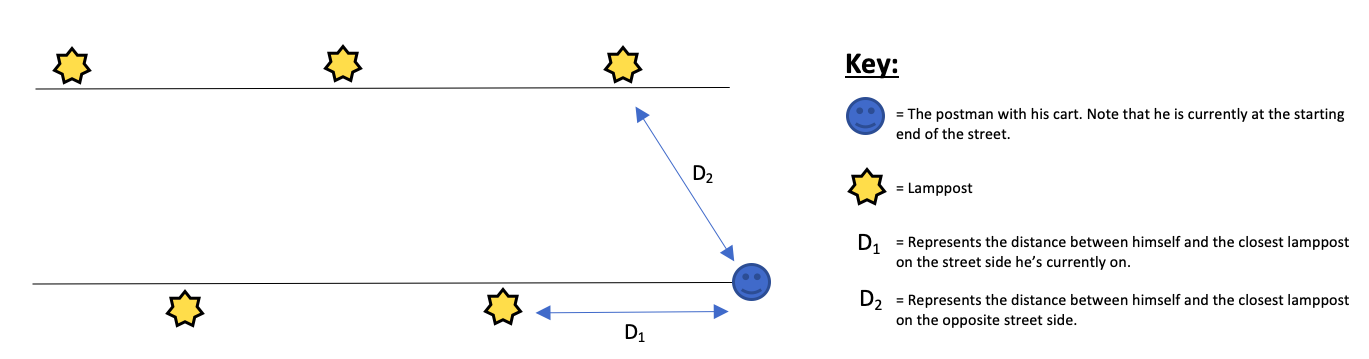
\includegraphics[width = 430pt]{Images/DiagramIllustratingTheTwoDistancesTheAlgorithmIsComparing.png}
    \caption{Diagram Illustrating The Two Distances The Algorithm Is Comparing}
    \label{fig:Diagram illustrating the two distances the algorithm is comparing}
    \end{figure}

    \item Next, he checks if there exists any houses on either side of the road between his starting position, and the lamppost he’s currently at. If houses exist, he then checks how much post is due at each house. If the amount of post due exceeds the max capacity of his sack, he will end up performing multiple trips to and from his cart, until all houses have received their post.
    \item When he performs a trip delivering post to the houses, the algorithm treats each house as a point, and connects the points up, forming a ‘polygon’. He then travels along this ‘polygon’ delivering the post. Please note however, that in the case that he makes a delivery to only houses on the roadside he’s currently on, he’ll travel along a straight line instead.
    \item Once he delivers to all houses between the starting point and the lamppost he’s currently at, the algorithm then finds the next closest lamppost that’s also ahead of the current carts position. It then checks for any houses due post between these two ‘points’, and delivers to any houses that have post due there. 
    \item After all these houses have received their post, the postman will then move to this next lamppost with his cart, chain up, and repeat this process. He’ll keep doing this until he gets to the final lamppost, and delivers to the houses that may exist between the last lamppost and the end of the street.
    \item Once the postman has delivered to the entire street, the algorithm will return the total distance travelled by the postman.
\end{enumerate}
     \\
\\
From the total distances travelled by the postman in each of our three models, time taken can be calculated (where walking speed of the postman is assumed constant) and compared between each.  This lets us analyse which route is most effective for a variety of streets with different sets of parameters.


\section{Discussion and Conclusion}

As our final models allow for different parameters to be inputted, we do not have a general set of times that tell us which route is quickest.This is more beneficial as no two roads are the same. A rural area for example will have different roads to that of a urban area (all parameters will be different). Thus, we have chosen to have different output times depending on the street's parameters, as well as the model used. This means that depending on the road, any of these models could work out to be the most time efficient. We have shown below our results for two different roads.  

\subsection{Urban Road}
Typically, a street in an urban area will have houses, as well as lampposts, at a fairly consistent distance apart. For example, we are going to take a street with 10 houses at a 10m width on each side. Lampposts are at points 0, 30, 60 and 90 metres on each side of the street (with reference to the start of each side of the street). Amount of mail to be delivered to each house has been picked at random (as this will be consistently changing each day the postman delivers to a street). We are going to take the width of the street to be 10 metres, and that the postman can carry 15 deliveries at once. 
\\
When running the init python file, we achieved the following results for this particular urban street shown in Figure \ref{fig:Urban Street Results}. 

\begin{figure}[H]
\centering
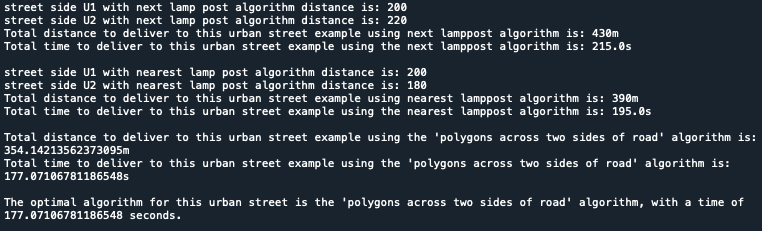
\includegraphics[width = 430pt]{Images/UrbanStreetResults.png}
\caption{Urban Street Results}
\label{fig:Urban Street Results}
\end{figure}

This shows that the 'polygons across two sides of road' (model 3) was quickest for this particular urban street, with a time of 158.5seconds.  

\subsection{Rural Road}
A rural street will consist of very different parameters compared to an urban street. Therefore, the parameters that we passed in changed drastically shown in Figure \ref{fig:rural street parameters}. 

\begin{figure}[H]
\centering
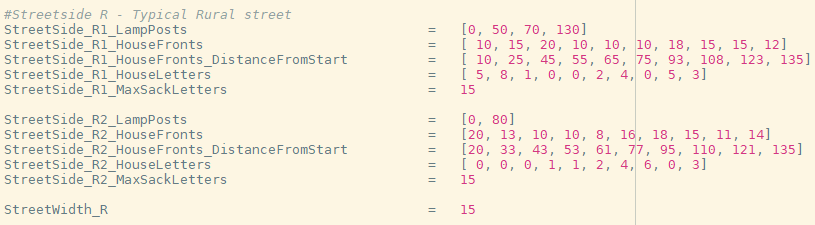
\includegraphics[width = 430pt]{Images/RuralStreetParameters.png}
\caption{Rural Street Parameters}
\label{fig:rural street parameters}
\end{figure}


We passed these parameters to find the best route for the postman delivering to this rural street. The optimal route was from model 3 - the 'polygons across two sides of road' algorithm. This gave a time of 234.1seconds shown below in Figure \ref{fig:rural street results}. 

\begin{figure}[H]
\centering
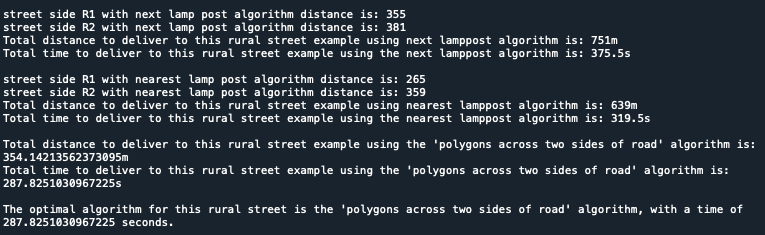
\includegraphics[width = 430pt]{Images/RuralStreetResults.png}
\caption{Rural Street Results}
\label{fig:rural street results}
\end{figure}

\subsection{Overall Results}
Sections 4.1 and 4.2 take examples of a possible urban and rural street respectively. Note that there is an infinite number of possible road structures. Amount of mail that each house receives will also vary so a postman's route is never going to be the same. The idea of our algorithm is that the postman can change the parameters depending on the road he is on, and also depending on the amount of mail each house needs. Thus, allowing him to choose which of the three routes to follow depending on these factors. Even though it appears that model 3 is best, this might not be the case for different urban and rural streets (where parameters are different from those used above). 

These results are accurate (under assumptions) for a single road only. If we had a system of multiple streets all connected together, results may fluctuate. Consider a case where model 3 is quickest. If the postman needs to get back to his start position to get to the next delivery street, then this model may not be quickest. Models 1 and 2 both have the postman looping back to the start position, rather than ending on the last delivery house at the far end of the street, as in model 3. This shows that the postman's position, after delivering to a whole street, will be a factor when considering multiple streets. 

\subsection{Merits}
Our algorithm allows for you to model your own street allowing the user to get a fair representation of spacing and time, rather than our code only allowing for one location. Our initial algorithms we developed assumed every house was delivered to, whereas this algorithm, based off inputs, chooses to deliver to set houses, skip past it or go back to the cart. Similarly this lets you deliver multiple letters to different houses depending on user input, the rules do not assume every house is delivered to nor do they assume that it is a set number of letters removed at each house. An essential addition to resemble the rules and objectives that a postman would have to follow throughout his shift. 

Another advantage of our updated algorithms is the removal of distances of driveways and pavements. Instead, the distance between houses is set from door to door. The sum of all driveway lengths will be a constant value, independent of the route taken. As a result, there is no need to include this in calculations to compare overall times between each model. This removes any error when worrying about the shape of the street. 

\subsection{Limitations and improvements}
Although flexible, the rules and assumptions we have made have limitations. Two of our finished set of rules calculate the distance by assuming the post mans route would be down one side of the street and up the other. This works fine with a single, perfectly straight street, as distances that are inputted make the shape of a street irrelevant However, when adding another street to the model, it would increase the distance largely through inefficient routing. In simplistic terms our route would force the postman to go up and back down the street, then back up, for the next street creating a very inefficient way to deliver to the second street. The position of the postman after finishing one street, in relation to where the start of the next street is, would become an important factor. 
For a future model we would create an algorithm that includes multiple streets, connected in different ways. Depending on how these roads are connected will influence whether the postman completes he route street by street, or another, more efficient way (that would need to be determined).  

We have also assumed that the walking speed remains constant despite variations in human error/ weight of letters he is carrying/ carts weight when pushing it. Although taking this into account would be an improvement of our algorithm it will only result in an inconsequential change in our outputted times. 

We assumed that each house has its door positioned at the end of its width which is unrealistic, so the position of each house's door, with respect to its width, could be taken as a random variable, making our results more accurate. A further improvement would be to randomise the amount of mail each house receives, between zero and a maximum value, to make it more realistic. 

Lastly, we have also not included the time it takes to lock up the cart to a lamppost. Next time, we should set a constant time to lock up the cart. Multiplying by the number of times the cart needs to be locked up, and adding this to the total time would give better results. This might have an overall effect on which route is quickest. The most appropriate route will depend on the total time to cover the total distance travelled, but also dependent on the number of times the cart needs to be locked up. 

\subsection{Validation}
In each of these streets, we only considered 10 houses on each side. This is so that we were able to determine if the code was working as expected. Note that in the "SideOfStreetModels" python module, there is actually more streets with different parameters. Expected results for some of these other streets are found in the init module, in commented tables. These were used initially as a check to ensure that our code was producing the correct results. 

Please see figures 6 to 8 (in our appendix) which show our expected results (done by hand) for the urban street using each algorithm. These match the results in our algorithm. As the code works as expected for the urban street, it will also work as expected for the rural street, as well as any other street with different parameters. This validates that our code works correctly. 

To validate our results to a real postman delivering mail to a street, we would need to conduct an experiment where we record the time it takes for an actual postman to complete deliveries. We could then record the difference between each set of results to see if our results, for any model, are valid. 


\section{References}
From introduction \textbf{(1)} https://freakonometrics.hypotheses.org/53694

From introduction \textbf{(2)} http://www.suffolkmaths.co.uk/pages/Maths%20Projects/Projects/Topology%20and%20Graph%20Theory/Chinese%20Postman%20Problem.pdf

\section{Appendix}
\begin{figure}[H]
\centering
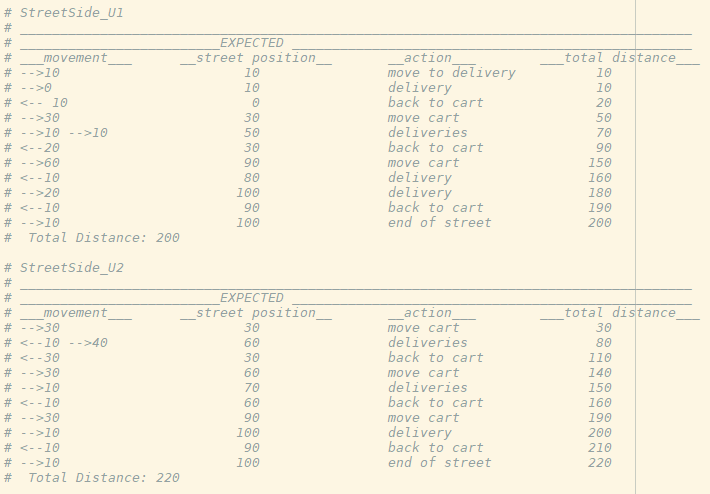
\includegraphics[width = 430pt]{Images/UrbanStreetExpectedResultsNextLampPost.png}
\caption{Rural Street Expected Results using Next Lamppost Algorithm}
\label{fig:rural street expected results using next lamppost algorithm}
\end{figure}

\begin{figure}[H]
\centering
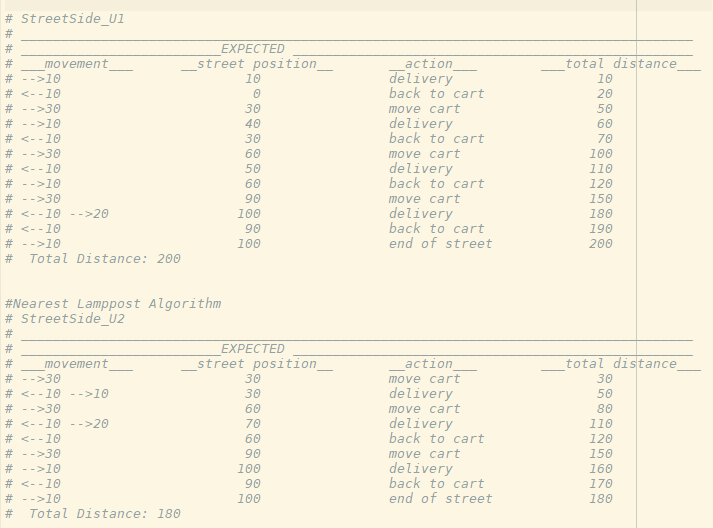
\includegraphics[width = 430pt]{Images/UrbanStreetExpectedResultsNearestLampPost.png}
\caption{Rural Street Expected Results using Nearest Lamppost Algorithm}
\label{fig:rural street expected results using nearest lamppost algorithm}
\end{figure}


\end{document}


